\documentclass[aspectratio=1610]{beamer}
\usetheme{lucid}
\usepackage[utf8]{inputenc}
\usepackage{amsmath, xcolor, graphicx}

\definecolor{newgray}{RGB}{230, 230, 255}

\setbeamersize{text margin left=2cm,text margin right=2cm}


\title{The Cubic Spline Interpolation}
\subtitle{MA3105 Group project and Presentation}
\author{Rudra Mukhopadhyay}

\begin{document}
\frame{
 \titlepage
}

\frame {
 \frametitle{Goal}
    \begin{itemize}
        \item Presenting the cubic spline interpolation technique and the associated error analysis.
        \item Finding the spline interpolant of $f(x) = e^x$ on $[-1, 1]$ with three different meshes.
        \item Comparing the technique with linear and quadratic LIPs.
    \end{itemize}
}

\section{Introduction}

\frame {
 \frametitle{Spline interpolation}
    \begin{itemize}
        \item Over an interval $\Omega = [a,b] (a,b \in \mathbb{R})$, a few points and the corresponding functional values are given.
        \item $\Pi := \{a = x_0, x_1, \dots, x_n = b\}$. $\forall x_i \in \Pi$, $x_i$ is called a \emph{knot}.
        \item Instead of fitting a polynomial with degree $\leq n+1$, we fit a polynomial $s_i$ of degree $m$ over every interval $[x_i, x_{i+1}], i = 0, 1, \dots, n-1$.
        \item Each of $s_i, i = 0, 1, \dots, n-1$ is called a \emph{spline}.
    \end{itemize}
} 

\frame{
 \frametitle{A simple linear spline}
    \begin{itemize}
        \item Connecting two consecutive points in the mesh $\Pi$ with a straight line.
        \item $s_L(x) = \dfrac{x_i - x}{x_i - x_{i-1}}f(x_{i-1}) + \dfrac{x - x_{i-1}}{x_i - x_{i-1}}f(x_i)$\\
        \hspace{6 cm}
        $x \in [x_{i-1}, x_i], i = 1, \dots, n$
        \item With $f \in C^2(\Omega)$ and $h:=\max{h_i}$, $||f-s_L||_\infty \leq \dfrac{1}{8}h^2(||f''||_\infty)$
    \end{itemize}
}

\section{Pros}
\frame{
 \frametitle{Why spline interpolation}
    \begin{itemize}
        \item Low computational cost
        \item Less possibility of over-fitting
        \item Customizability in terms of \emph{smoothness}
    \end{itemize}
}

\section{About Cubic spline}
\frame{
 \frametitle{The cubic spline}
    $f \in C[a,b]$ and the mesh is given by $\Pi$ over the interval $\Omega$.\\
    Consider $\mathcal{S} := \{s|s \in C^2(\Omega)\}$ such that-
    \begin{enumerate}
        \item $s(x_i) = f(x_i), \forall x_i \in \Pi$
        \item $deg(s) \leq 3$ on $[x_{i-1}, x_i], i = 1, \dots, n$
    \end{enumerate}
}

\frame{
 \frametitle{Finding constraints}
    \begin{itemize}
        \item On each $[x_{i-1}, x_i]$, $s_i := a_ix^3 + b_ix^2 + c_ix + d$\\ $\implies 4n$ unknown coefficients to solve for.
        \item $2n$ constraints: $s_i(x_i) = f(x_i), s_i(x_{i+1}) = f(x_{i+1}); i = 0, \dots, n-1$
        \item $2(n-1)$ constraints:\\
        $s'_i(x_{i+1}) = s'_{i+1}(x_{i+1}),$\\
        $s''_i(x_{i+1}) = s''_{i+1}(x_{i+1}), i = 0, \dots, n-2$
        \item 2 boundary conditions: four major categories.
    \end{itemize}
}

\section{Different classes}
\frame{
 \frametitle{Different classes}
    \begin{itemize}
        \item \color{newgray}{Natural cubic}\\
        \hspace{1cm}
        \color{white}{$s''(x_0) = s''(x_n) = 0$}
        
        \item \color{newgray}{Clamped spline}\\
        \hspace{1cm}
        \color{white}{$s'(x_0) = f'(x_0), s'(x_n) = f'(x_n)$\\
        \hspace{1cm}
        Or, $s''(x_0) = f''(x_0), s''(x_n) = f''(x_n)$}
        
        \item  \color{newgray}{Not-a-knot spline}\\
        \hspace{1cm}
        \color{white}{$s'''(x_1) = s'''(x_2), s'''(x_{n-1}) = s'''(x_{n-1})$}
        
        \item \color{newgray}{Periodic spline}\\
        \hspace{1cm}
        \color{white}{$s(x_0) = s(x_n), s'(x_0) = s'(x_n)$}
    \end{itemize}
}

\section{Solving the spline}
\frame{
 \frametitle{Deriving the equations}
    \begin{enumerate}
        \item $s$ be the spline interpolate over $\Omega$.
        \item $\sigma_i := s''(x_i)$ over the interval $[x_i,x_{i+1}]$
        \item $s''$ is linear. Thus, $s''(x) = \dfrac{x_{i+1}-x}{h_i}\sigma_i + \dfrac{x-x_i}{h_i}\sigma_{i+1}, h_i:=x_{i+1}-x_i$
        \item $s''$ is integrated twice, with the constraints $s(x_i) = f(x_i), s(x_{i+1} = f(x_{i+1})$. \item $s'$ has to be continuous over $\Omega$\\ 
        $\implies s'_i(x_{i+1}) = s'_{i+1}(x_{i+1}), i = 0,\dots, n-2$ 
    \end{enumerate}
}

\frame{
 \frametitle{Deriving the equations}
    The system of linear equations, given by-\\
    $
    h_{i+1} \sigma_i + 2(h_{i+2} + h_{i+1})\sigma_{i+1} + h_{i+2}\sigma_{i+2} =$\\
    \hspace{2 cm}
    $6\Big(\dfrac{f(x_{i+2})-f(x_{i+1})}{h_{i+2}}-\dfrac{f(x_{i+1})-f(x_i)}{h_{i+1}}\Big)$\\
    \hspace{6 cm}
    For $i=0,\dots,n-2$\\
    - a \emph{tridiagonal system}, is to be solved.
}

\frame{
 \frametitle{Solving a tridiagonal system}
    \begin{itemize}
        \item Algorithm:
        \begin{itemize}
            \item Thomas algorithm.
            \item $\mathcal{O}(n)$
        \end{itemize}
        \item Non-singularity:
        
    \end{itemize}
}

\section{Error analysis}
\frame{
 \frametitle{Error bound}
    \begin{itemize}
        \item \color{newgray}{Natural cubic}\\
        \color{white}{
        \begin{itemize}
            \item $||f(x)-s_N(x)||_\infty \leq \mathcal{K}_N h^2$
            \item $h:= \max_{\Omega}(x_{i+1}-x_i), i=0, \dots, n-1$
            \item $\mathcal{K}_N$ is dependent on $||f^{(4)}(x)||_\infty$.
            \item The rate of convergence increases for clamped/ complete cubic.
        \end{itemize}
        }
        \item \color{newgray}{Clamped cubic}\\
        \color{white}{
        \begin{itemize}
            \item $||f(x)-s_C(x)||_\infty \leq \mathcal{K}_C h^4$
            \item The optimum value\footnote{Theorem 5. Hall, Meyer (1976)} for $\mathcal{K}_C = \frac{5}{384}||f^{(4)}||_\infty$  
        \end{itemize}
        }
    \end{itemize}
}

\frame{
 \frametitle{An intuitive justification}
 \framesubtitle{For the error bound in natural cubic}
    \begin{enumerate}
    \item Assumption: the mesh is uniform
        \item $||f-s_N||_\infty = ||f-g+g-s_N||_\infty \leq ||f-g||_\infty + ||g-s_N||_\infty$
        \item $deg(g) \leq 3$ and $g''(a) = g''(b) = 0, f(x_i)=g(x_i) \forall i \in \{0, \dots, n\}$
        \item Thus, $||g-s_N||_\infty = \mathcal{O}(h^4)$
        \item Because of (3), $||f''-g''||_\infty = \max{\{||f''(a)-g''(a)||, ||f''(b)-g''(b)||\}} = c (\neq 0)$
        \item $||f-g||_\infty =\mathcal{O}(h^2)$
    \end{enumerate}
}

\section{Solving the problem}
\frame{
 \frametitle{Plots and errors}
 \framesubtitle{Natural cubic spline}
    \begin{figure}
        \centering
        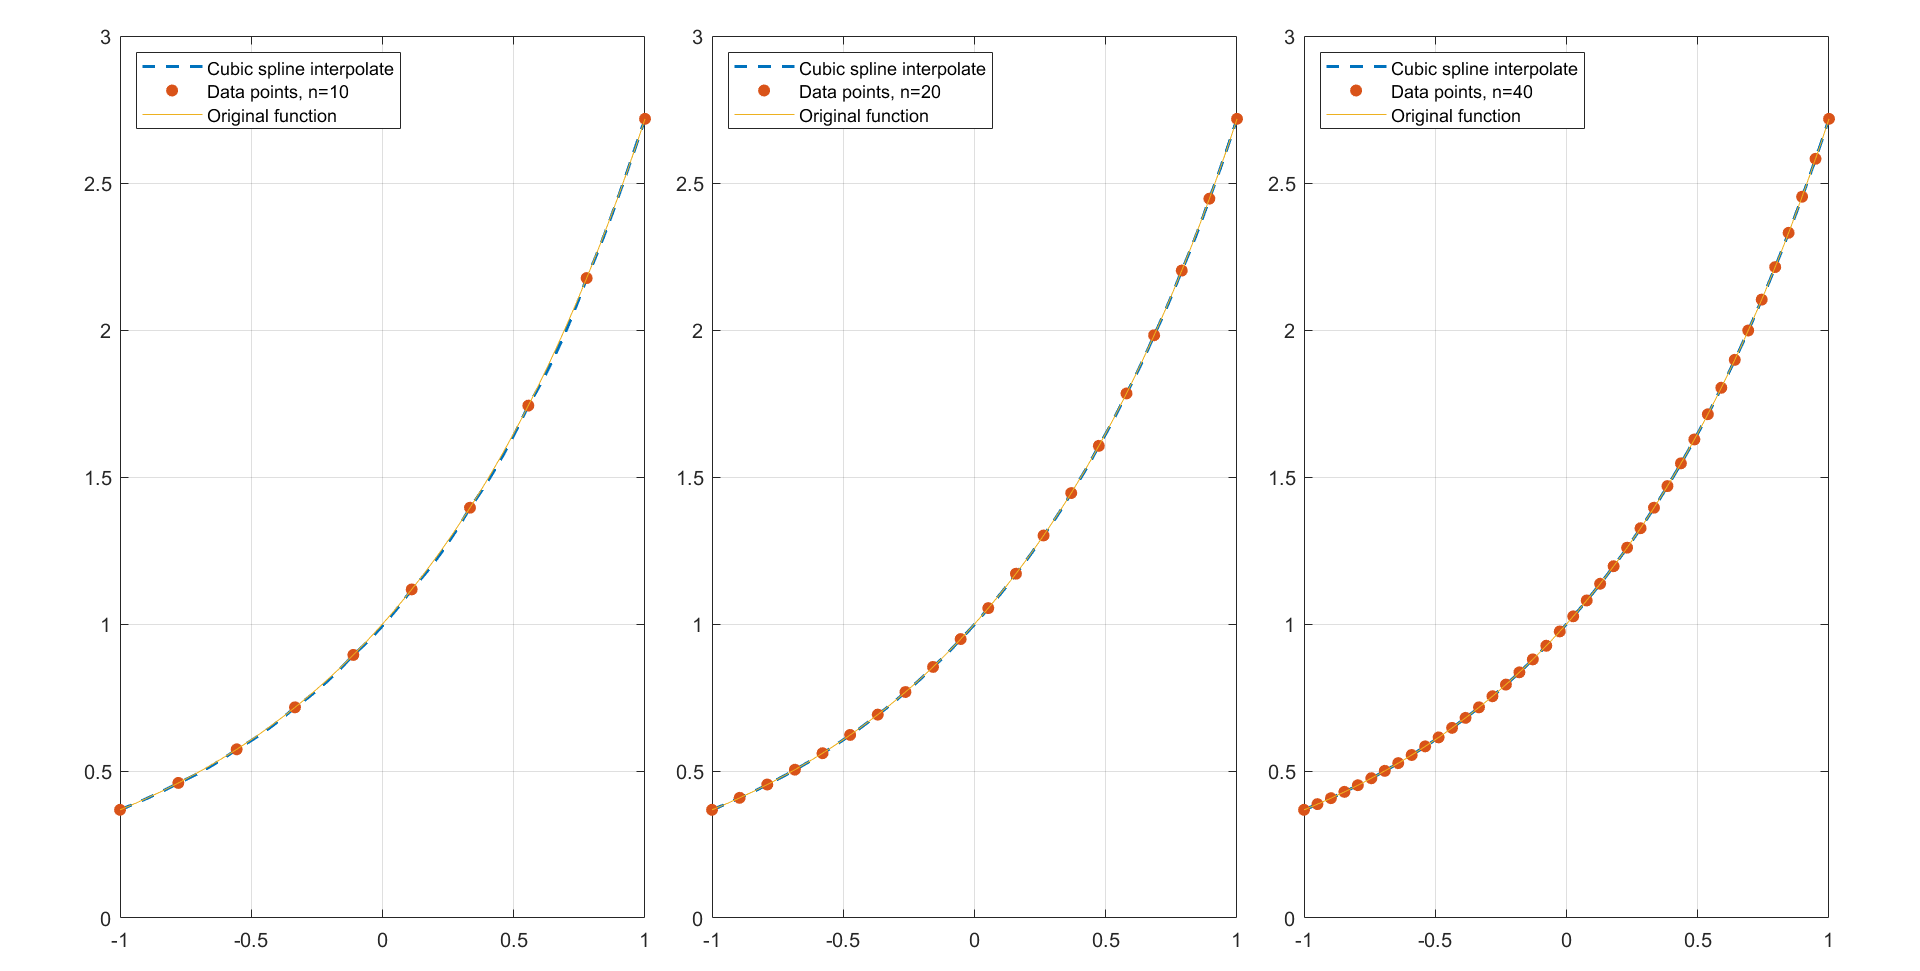
\includegraphics[scale = 0.22]{nat_cub.png}
    \end{figure}
}

\frame{
 \frametitle{Plots and errors}
 \framesubtitle{Clamped cubic spline}
    \begin{figure}
        \centering
        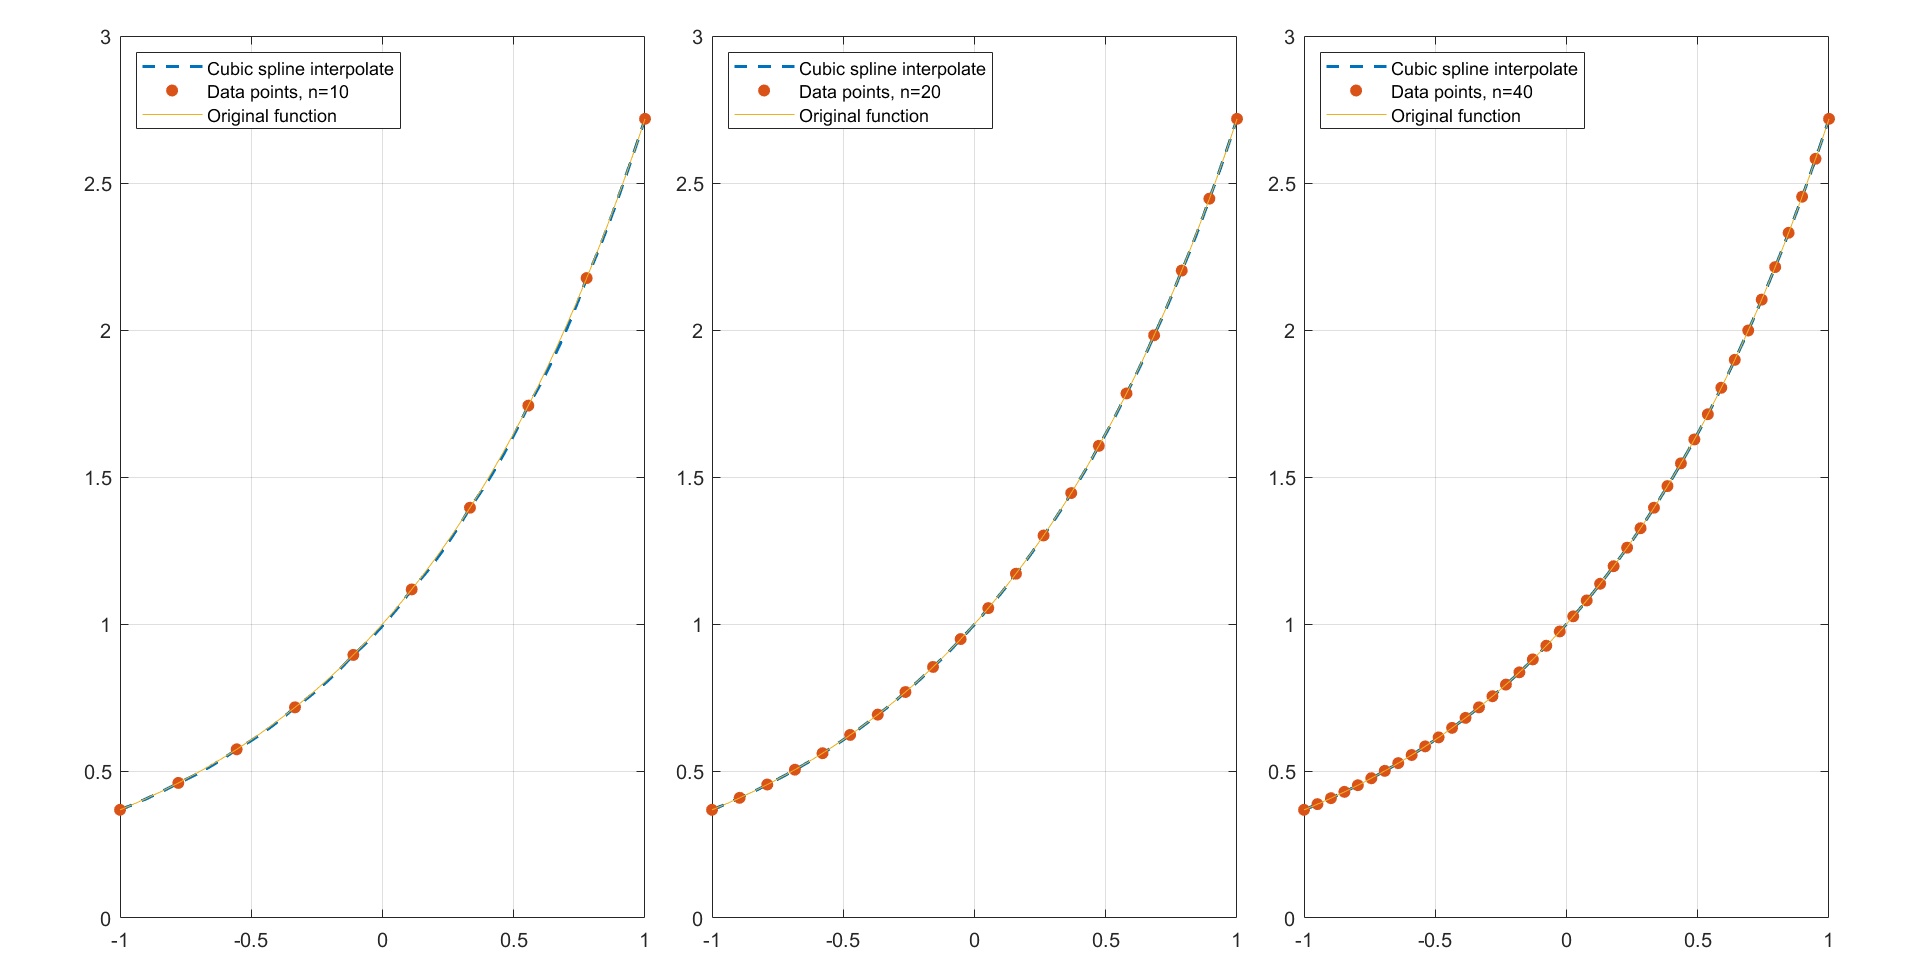
\includegraphics[scale = 0.22]{clmp_cub.png}
    \end{figure}
}

\frame{
 \frametitle{Plots and errors}
    \large{$L_\infty$ norm of the error:}\\
     \begin{table}
         \centering
         \begin{tabular}{|c|c|c|}
            \hline
            n & Natural & Clamped\\
            \hline
            \hline
            10 & 0.0155 & 0.0138\\
            \hline
            20 & 0.0039 & 0.0036\\
            \hline
            40 & 9.76e-4 & 8.95e-4\\
            \hline
         \end{tabular}
     \end{table}
     
     \large{$L_2$ norm of the error:}\\
     \begin{table}
         \centering
         \begin{tabular}{|c|c|c|}
            \hline
            n & Natural & Clamped\\
            \hline
            \hline
            10 & 0.0762 & 0.0783\\
            \hline
            20 & 0.0182 & 0.0184\\
            \hline
            40 & 0.0044 & 0.0045\\
            \hline
         \end{tabular}
     \end{table}
}

\section{Comparing with LIP, QIP}
\frame{
 \frametitle{Comparison with Lagrangian}
    \begin{figure}
        \centering
        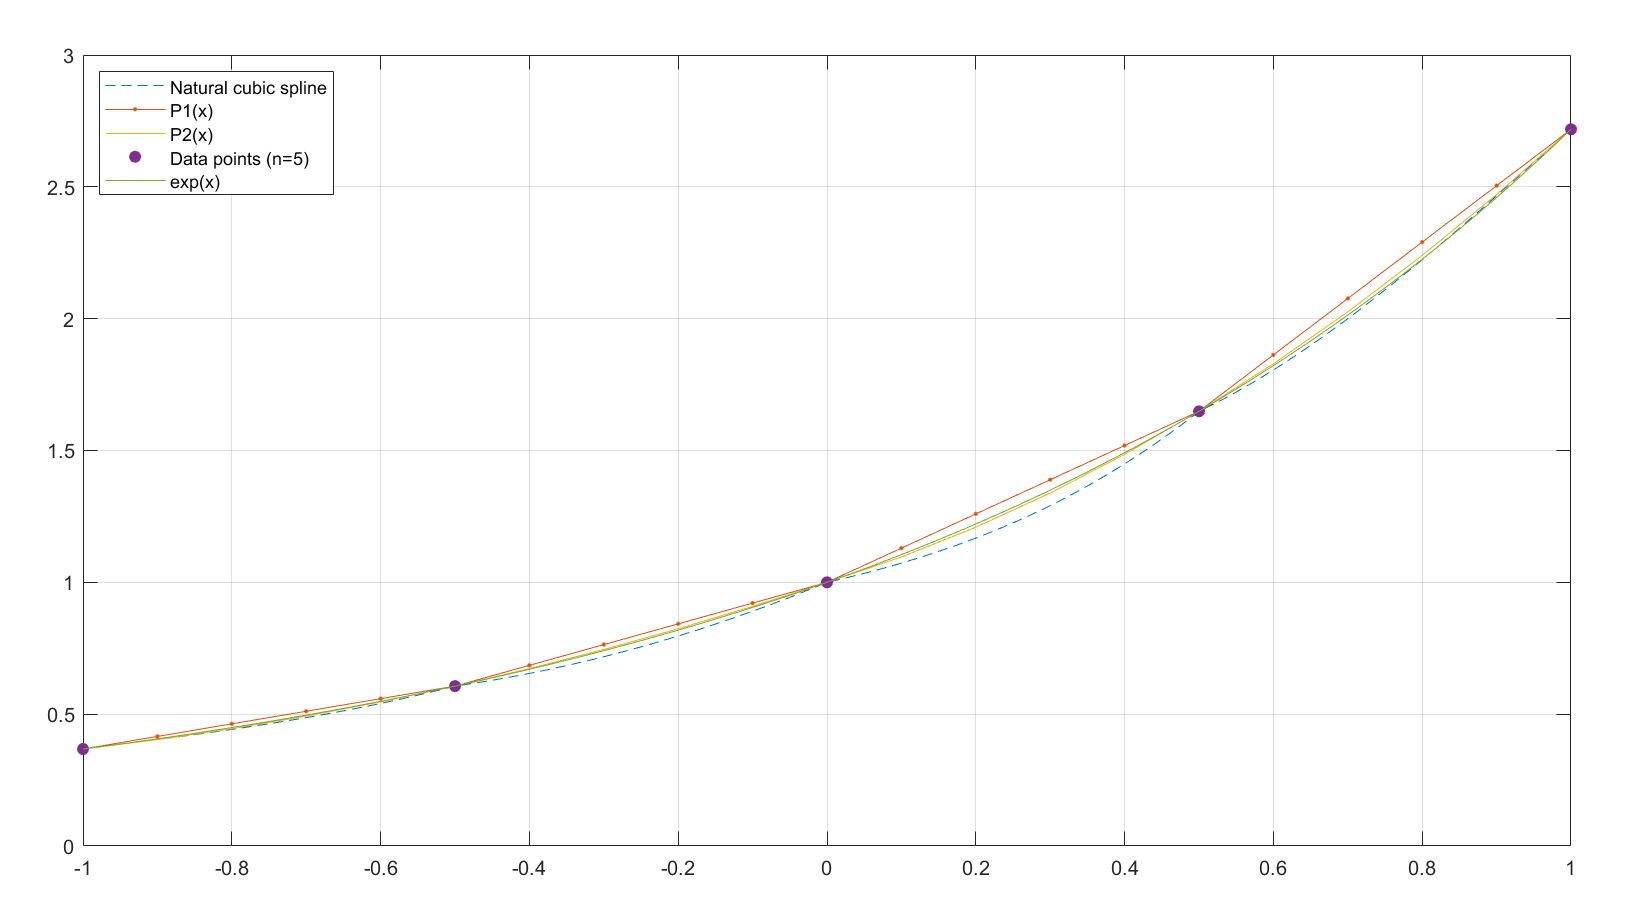
\includegraphics[scale = 0.23]{comp_5.png}
    \end{figure}
}
 
\frame{
 \frametitle{Comparison with Lagrangian}
 \framesubtitle{With different mesh density}
 \large{$L_\infty$ norm of the error}
    \begin{table}
        \centering
        \begin{tabular}{|c|c|c|c|}
            \hline
            n & $P_1(x)$ & $P_2(x)$ & $s_N(x)$\\
            \hline
            \hline
            5 & 0.064917 & 0.014416 & 0.059208\\
            \hline
            10 & 0.014825 & 0.001189 & 0.015507\\
            \hline
            15 & 0.005478 & 0.000391 & 0.007013\\
            \hline
            20 & 0.000690 & 0.000075 & 0.003943\\
            \hline
            25 & 0.000000 & 0.000047 & 0.002547\\
            \hline
            30 & 0.000000 & 0.000047 & 0.001778\\
            \hline
            35 & 0.000000 & 0.000031 & 0.001295\\
            \hline
            40 & 0.000000 & 0.000005 & 0.000976\\
            \hline
        \end{tabular}
    \end{table}
}   

\frame{
 \frametitle{Comparison with Lagrangian}
 \framesubtitle{With different mesh density}
 \large{$L_2$ norm of the error}
    \begin{table}
        \centering
        \begin{tabular}{|c|c|c|c}
            \hline
            n & $P_1(x)$ & $P_2(x)$ & $s_N(x)$\\
            \hline
            \hline
            5 & 0.135386 & 0.032530 & 0.337271\\
            \hline
            10 & 0.026198 & 0.002383 & 0.076190\\
            \hline
            15 & 0.010887 & 0.000749 & 0.032801\\
            \hline
            20 & 0.001568 & 0.000132 & 0.018169\\
            \hline
            25 & 0.000000 & 0.000087 & 0.011525\\
            \hline
            30 & 0.000000 & 0.000094 & 0.007955\\
            \hline
            35 & 0.000000 & 0.000068 & 0.005819\\
            \hline
            40 & 0.000000 & 0.000012 & 0.004442\\
            \hline
        \end{tabular}
    \end{table}
}

\frame{
 \frametitle{Remark}
    \begin{itemize}
        \item The error bound of a Lagrangian interpolate converges faster than a cubic spline interpolate.
        \item On a uniform mesh with $n$ points $||f-p|| \leq \mathcal{K_L}|\pi_{n+1}(x)| = \mathcal{O}(h^{n+1})$, where $h:=\frac{b-a}{n-1}$.
    \end{itemize}
}
\end{document}
